\documentclass{article}
\usepackage[hidelinks]{hyperref}
\usepackage{xeCJK}
\usepackage{indentfirst} 
\usepackage{geometry}
\usepackage{framed}
\geometry{a4paper,top=2.54cm,bottom=2.54cm,left=3.18cm,right=3.18cm}
\parindent 2em % 段首缩进
\pagenumbering{roman}

\begin{document}

\author{林庆毫}
\title{关于毕业论文模板的说明}
\maketitle
\tableofcontents
\newpage
\pagenumbering{arabic}

\section{模板来源}
https://github.com/ahhylau/shuthesis

\section{模板编译环境}
建议在 Linux 下安装 texlive-full 和 latexmk 等环境后根据 shuthesis.pdf 教程进行编译。
\begin{framed}
    sudo apt install texlive-full latexmk -y
\end{framed}

如果选择在 Windows 环境下编译,texlive 无法正常编译 main.tex 中 makefirstpage,需要手动跳过各种错误。可以将 makefirstpage 注释,完稿后通过跳过错误的方式进行完整的编译,或另用 pdf 工具拼接上封面页。

\section{模板中存在的问题}
英文参考文献,若作者多于 3 人,有的会出现中文的 “等”。
\begin{figure}[h]
    \centering
    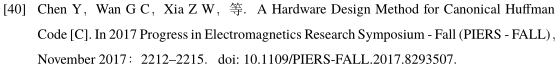
\includegraphics[scale=0.7]{../assets/images/2021-05-27-10-43-57.png}
\end{figure}

出现原因:
模板中判断参考文献是中文还是外文的方法是:language 字段为空=英文;language 字段不为空=中文。上图文献在 refs.bib 中有 language = \{en\} 字段,导致误认为属于中文文献。

解决方案:
能力有限,这个问题不那么好解决,因此只能采用一个妥协方案。
refs.bib 中所有的英文文献都不要带 language 字段,反之中文文献都加上。

\end{document}